%!TEX root = ../thesis.tex

\section{学習フェーズ}

  学習フェーズで使用するルールベース制御器を\figref{Fig:okada_rule-based_contoroller}に示す.ルールベース制御器は,引き紐に取り付けられたポテンショメータからのリンクの角度を入力とし,ルールに従いロボットの行動を選択する.ルールベース制御器からの出力を\tabref{tab:actions_control_parameters}に示す.なお,並進速度は0.1 \,[m/s]で一定である.

  \begin{figure}[h]
    \centering
    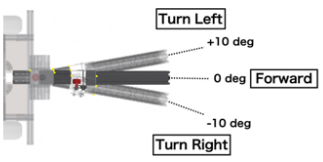
\includegraphics[keepaspectratio, scale=0.70] {images/okada_rule-based_contoroller.png}
    \caption{Action according to angles of the joint \cite{okada}}
    \label{Fig:okada_rule-based_contoroller}
  \end{figure}

  \begin{table}[ht]
    \caption{The control rule and action parameters}
    \label{tab:actions_control_parameters}
    \centering
    \begin{tabular}{|c|c|c|c|}
    \hline
    \textbf{Action} & \textbf{Control rule} & \textbf{Linear velocity} & \textbf{Angular velocity} \\ 
    \hline
    Turn Left & $\theta_{\mathrm{yaw}} > 10 \, \mathrm{deg}$ & 0.1 \,m/s & 0.2 \,rad/s \\ 
    \hline
    Forward & $-10 \, \mathrm{deg} < \theta_{\mathrm{yaw}} < 10 \, \mathrm{deg}$ & 0.1 \,m/s & 0 \,rad/s \\ 
    \hline
    Turn Right & $\theta_{\mathrm{yaw}} < -10 \, \mathrm{deg}$ & 0.1 \,m/s & -0.2 \,rad/s \\ 
    \hline
    \end{tabular}
    \end{table}
  
\newpage